\documentclass[]{scrartcl}

\usepackage{hyperref}
\usepackage{graphicx}
%\graphicspath{./Images/}
\usepackage{wrapfig}
\usepackage{paralist}
\usepackage{microtype}

\setlength{\parindent}{0em}
\setlength{\parskip}{1ex}

%opening
\title{Installations in Manjaro 21.2}
\author{Pablo Adames}

\begin{document}
	
	\maketitle
	
	\begin{abstract}
		Reinstalled Manjaro 21.2 on /dev/sdb following Manjaro Forum recommendations.
		Windows continues installed on /dev/sda.
		The dual boot continues to be handled well by the boot loader.
	\end{abstract}
	
	\section{Development tools}
	
	\begin{verbatim}
		sudo pacman -Syyu
		sudo pacman -S base-devel
	\end{verbatim}
	
	\section{R}
	
	\begin{verbatim}
		pamac install intel-mkl
		sudo find / -type d -iname mkl 2>/dev/null
	\end{verbatim}
	
	The output of the latter was
	\begin{verbatim}
		/opt/intel/mkl
	\end{verbatim}
	
	So I set the environment variable needed for the build step:
	
	\begin{verbatim}
		export MKLROOT="/opt/intel/mkl"
	\end{verbatim}
	
	After that the last step is:
	
	\begin{verbatim}
		pamac build r-mkl
	\end{verbatim}
	
	To find out what configuration I have:
	\begin{verbatim}
		/opt/intel/mkl/bin/mkl_link_tool
	\end{verbatim} 
	
	
	\section{RStudio}
	
	Starting from home:
	
	\begin{verbatim}
		mkdir Downloads/RStudio
		cd Downloads/RStudio
		git clone https://aur.archlinux.org/r-studio-for-linux-bin.git
		cd r-studio-for-linux-bin/
		updpkgsums
		makepkg -si	
	\end{verbatim}
	
	This is a deceivingly namesake of the real RStudio. It is a utility to manage the file system.
	Apparently there is no easy way to install RSTudio in Manjaro.
	
	So I removed it from the Manjaro Software utility.
	
	Retrying:
	
	\begin{verbatim}
		mkdir Downloads/RStudio
		cd Downloads/RStudio
		git clone https://aur.archlinux.org/rstudio-desktop.git
		cd rstudio-desktop/
		updpkgsums
		makepkg -si	
	\end{verbatim}
	
	This had the error mentioned in \href{https://forum.manjaro.org/t/rstudio-on-pinebook-pro-aarch64/60827/6?u=padames}{Installing RStudio}. The responder states that the AUR repo does not have the dependencies necessary to build RStudio.
	
	\begin{figure}[!htb]
		\centering
		\caption{Error after executing \texttt{makepkg -si}}
		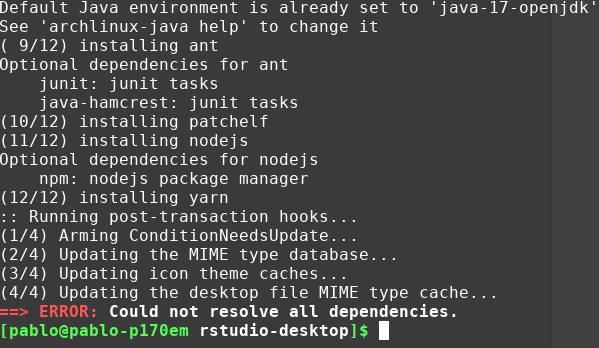
\includegraphics[width=0.45\textwidth]{Images/ErrorInstallingAUR.png}
	\end{figure}
	
	In my final attempt of the night I succeeded follwing the \textit{yay} route as described in \href{https://archived.forum.manjaro.org/t/using-the-statistical-package-r-in-manjaro-with-rstudio/484}{Manjaro Forum on RStudio-archived}. 
	It came down to doing a single command line:
	\begin{verbatim}
		yay -S rstudio-desktop-bin
	\end{verbatim}
	Of course, first I had to install yay (see \S\ref{sec:yay})
	
	The version installed was RStudio 2021.09.2
	
	\begin{figure}[!htb]
		\centering
		\caption{RStudio 2021.09.2 Build 382.}
		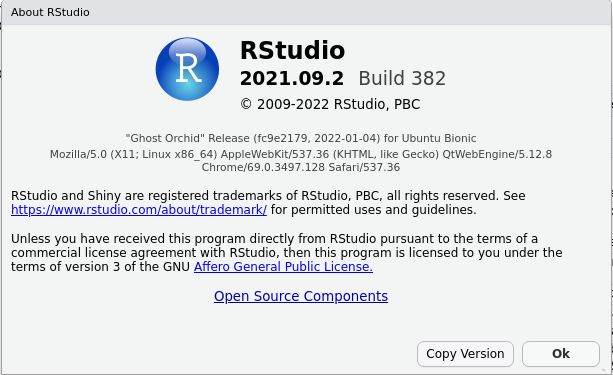
\includegraphics[width=0.45\textwidth]{Images/RStudioSplashWindowFeb07-2022.png}
	\end{figure}
	
	On October 12, 2022, I had to re-install RStudio with
	\begin{verbatim}
		yay -S rstudio-desktop-bin
	\end{verbatim}
	
	because when I tried to run RStudio there was a missing library error. 
	Re-installing seemed a reasonable solution, the package installed was rstudio-desktop-bin-2022.07.1.554-2 and \texttt{rstudio-desktop} was removed in the process.
	
	\section{Yay}
	\label{sec:yay}
	
	Followed directions from \href{https://www.tecmint.com/install-yay-aur-helper-in-arch-linux-and-manjaro/}{Installing Yay}
	
	\section{AUR}
	
	Enabled AUR in the Add/Remove Software to have access to the Arch Liux packages in Manjaro as suggested \href{https://forum.manjaro.org/t/dropbox-install-new-to-manjaro/9576/5}{here} while searching for a recipe to install Dropbox.
	
	\section{Date}
	
	On April, 17, 2022 Manjaro reported the wrong date after installing updates.
	Followed these steps to fix it (\href{https://archived.forum.manjaro.org/t/howto-get-your-time-timezone-right-using-manjaro-windows-dual-boot/89359}{get your time zone}):
	\begin{compactenum}
		\item  \verb|sudo timedatectl set-local-rtc 0|
		\item \verb|sudo systemctl enable --now systemd-timesyncd|
		\item \verb|sudo ln -sf /usr/share/zoneinfo/Canada/Mountain /etc/localtime|
	\end{compactenum}
	
	The region and time zone were found by first printing out all the time zones with:
	
	\verb|find /usr/share/zoneinfo/ -maxdepth 1 -type d|
	
	sample output:
	
	\begin{verbatim}
		/usr/share/zoneinfo/
		/usr/share/zoneinfo/Antarctica
		/usr/share/zoneinfo/Indian
		/usr/share/zoneinfo/Atlantic
		/usr/share/zoneinfo/America
		/usr/share/zoneinfo/Europe
		/usr/share/zoneinfo/Africa
		/usr/share/zoneinfo/Asia
		/usr/share/zoneinfo/Canada
		/usr/share/zoneinfo/right
		/usr/share/zoneinfo/Brazil
		/usr/share/zoneinfo/Arctic
		/usr/share/zoneinfo/Mexico
		/usr/share/zoneinfo/Chile
		/usr/share/zoneinfo/Pacific
		/usr/share/zoneinfo/Etc
		/usr/share/zoneinfo/Australia
		/usr/share/zoneinfo/US
		/usr/share/zoneinfo/posix
	\end{verbatim}
	
	Then the Canadian time zones with:
	
	\verb|ls /usr/share/zoneinfo/Canada|
	
	The output was:
	
	\begin{verbatim}
		Atlantic  Eastern   Newfoundland  Saskatchewan
		Central   Mountain  Pacific       Yukon
	\end{verbatim}
	
	This fixed my time zone issue today! Check with the command \texttt{date}.
	
	\section{Dropbox}
	
	Followed the \href{https://forum.manjaro.org/t/dropbox-install-new-to-manjaro/9576/5}{page in Manaro Forum}.
	
	First attempt here failed:
	\begin{small}
		\begin{verbatim}
			-> Downloading dropbox-lnx.x86_64-139.4.4896.tar.gz...
			% Total    % Received % Xferd  Average Speed   Time    Time     Time  Current
			Dload  Upload   Total   Spent    Left  Speed
			
			0     0    0     0    0     0      0      0 --:--:-- --:--:-- --:--:--     0
			2 96.1M    2 2578k    0     0  2757k      0  0:00:35 --:--:--  0:00:35 2755k
			9 96.1M    9 9310k    0     0  4804k      0  0:00:20  0:00:01  0:00:19 4804k
			16 96.1M   16 15.8M    0     0  5526k      0  0:00:17  0:00:02  0:00:15 5525k
			23 96.1M   23 22.6M    0     0  5890k      0  0:00:16  0:00:03  0:00:13 5888k
			30 96.1M   30 29.6M    0     0  6144k      0  0:00:16  0:00:04  0:00:12 6143k
			37 96.1M   37 36.2M    0     0  6248k      0  0:00:15  0:00:05  0:00:10 6900k
			44 96.1M   44 43.2M    0     0  6381k      0  0:00:15  0:00:06  0:00:09 6992k
			52 96.1M   52 50.2M    0     0  6484k      0  0:00:15  0:00:07  0:00:08 7048k
			59 96.1M   59 57.1M    0     0  6550k      0  0:00:15  0:00:08  0:00:07 7070k
			66 96.1M   66 63.7M    0     0  6566k      0  0:00:14  0:00:09  0:00:05 6982k
			73 96.1M   73 70.4M    0     0  6600k      0  0:00:14  0:00:10  0:00:04 7020k
			80 96.1M   80 77.5M    0     0  6657k      0  0:00:14  0:00:11  0:00:03 7040k
			87 96.1M   87 84.2M    0     0  6671k      0  0:00:14  0:00:12  0:00:02 6968k
			94 96.1M   94 90.9M    0     0  6685k      0  0:00:14  0:00:13  0:00:01 6927k
			100 96.1M  100 96.1M    0     0  6711k      0  0:00:14  0:00:14 --:--:-- 7017k
			-> Downloading dropbox-lnx.x86_64-139.4.4896.tar.gz.asc...
			% Total    % Received % Xferd  Average Speed   Time    Time     Time  Current
			Dload  Upload   Total   Spent    Left  Speed
			
			0     0    0     0    0     0      0      0 --:--:-- --:--:-- --:--:--     0
			100   473  100   473    0     0   2544      0 --:--:-- --:--:-- --:--:--  2556
			==> Validating source files with sha256sums...
			DropboxGlyph_Blue.svg ... Passed
			terms.txt ... Passed
			dropbox.service ... Passed
			dropbox@.service ... Passed
			==> Validating source_x86_64 files with sha256sums...
			dropbox-lnx.x86_64-139.4.4896.tar.gz ... Passed
			dropbox-lnx.x86_64-139.4.4896.tar.gz.asc ... Skipped
			==> Verifying source file signatures with gpg...
			dropbox-lnx.x86_64-139.4.4896.tar.gz ... FAILED (unknown public key FC918B335044912E)
			==> ERROR: One or more PGP signatures could not be verified!
			Failed to build dropbox
		\end{verbatim}
	\end{small}
	
	Second attempt was not what I expected because the installed program only opened a link to the Dropbox webpage.
	The I followed the download and build instructions from \href{https://help.dropbox.com/installs-integrations/desktop/linux-commands}{here}. 
	Then linked it to my free account which allows only three devices.
	
	\begin{figure}[!htb]
		\centering
		\caption{Connecting Dropbox client with server in the cloud. Removed the old reference to the previous Manjaro installation.}
		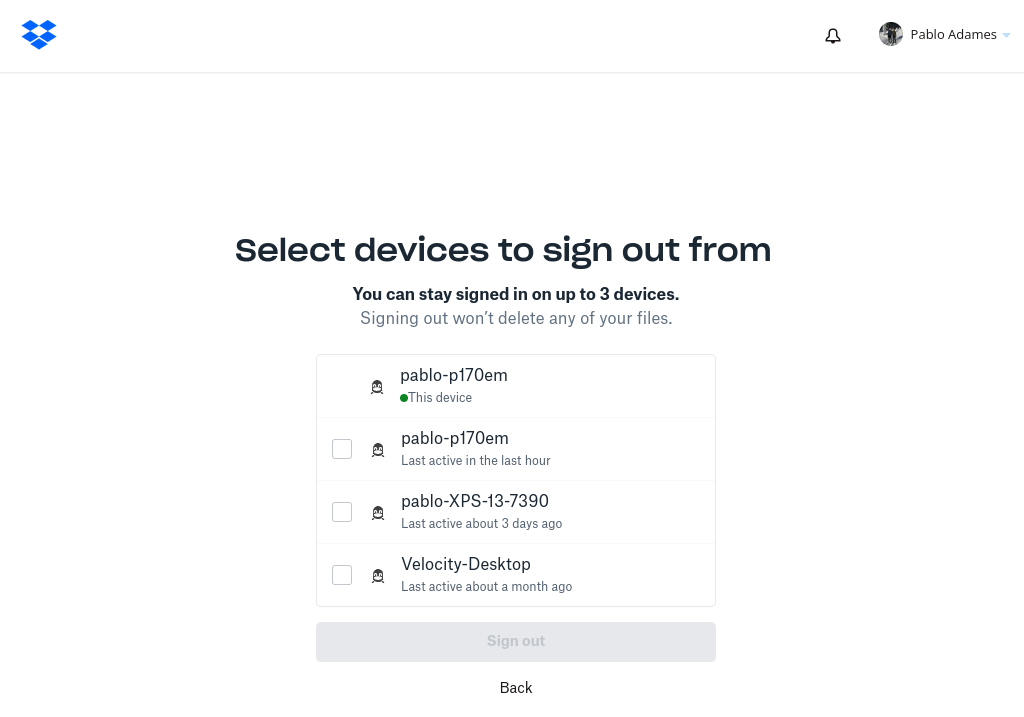
\includegraphics[width=0.8\textwidth]{Images/DropBoxSetUp.png}
	\end{figure}
	
	
	
\end{document}
